\documentclass[hyperref=colorlinks]{beamer}
\mode<presentation>
\usetheme{iclpt}
\setbeamertemplate{navigation symbols}{}
\setbeamertemplate{headline}{
\begin{beamercolorbox}[leftskip=.2cm,rightskip=.2cm,topskip=.2cm,ht=1.1cm,dp=0.1cm,wd=\textwidth]{institute in head/foot}
  
\includegraphics[height=1cm]{icl.pdf}
  \hfill
  
\includegraphics[height=1cm]{../Pics/CMS-Color.pdf}
\end{beamercolorbox}
}
\setbeamertemplate{footline}{
\begin{beamercolorbox}[ht=.55cm,dp=0.4cm,wd=\textwidth,leftskip=.3cm]{author in head/foot}%
  \begin{minipage}[c]{5cm}%
    \usebeamerfont{author in head/foot}
    \insertshortauthor 
    \insertshorttitle
    \end{minipage}\hfill%
  \insertframenumber{} / \pageref{lastframe}
  \hfill
  \begin{minipage}{6cm}
    \hfill
  \end{minipage}
\end{beamercolorbox}%
}

\usepackage{color}
\usepackage{tabularx,colortbl}
\usepackage{graphicx}
\usepackage{pdfpages}
\usepackage{feynmp}
\DeclareGraphicsRule{*}{mps}{*}{}

\title{\vspace{-0.2cm} First Look at Limits}
%\subtitle{Paper - HIG-13-030, PASs: HIG-13-013, HIG-13-018, HIG-13-028 \vspace{-0.7cm}}
\author[P. Dunne]{\underline{P. Dunne} }%\\ on behalf of the H$\rightarrow$invisible analysis groups} % A.M. Magnan and A. Nikitenko Joao Pela with \\ R. Aggleton, J. Brooke: Bristol \\ C.Asawangtrakuldee, Q.Li: Peking \\ P. Srimanobhas: Chulalongkorn \\ S. Kumar, K. Mazumdar: Mumbai}
\titlegraphic{
  \vspace{-0.7cm}
  %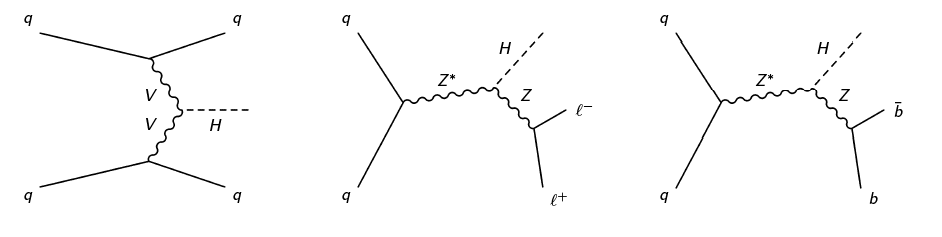
\includegraphics[width=\textwidth]{TalkPics/invcomb021213/feyndiags}
%% \begin{fmfgraph*}(100,70)
%%         \fmfleft{i1,i2}
%%         \fmfright{o1,o2,o3}
%%         \fmf{fermion}{i1,v1,o1}
%%         \fmf{fermion}{i2,v2,o3}
%%         \fmf{phantom,tension=4/5}{v1,v2}
%%         \fmffreeze
%%         \fmf{photon,label=$W,,Z$}{v1,v3}
%%         \fmf{photon,label=$W,,Z$}{v2,v3}
%%         \fmf{dashes}{v3,o2}
%%         \fmflabel{$q$}{i1}
%%         \fmflabel{$q$}{i2}
%%         \fmflabel{$q$}{o1}
%%         \fmflabel{$q$}{o3}
%%         \fmflabel{$H$}{o2}
%%       \end{fmfgraph*}
}
\date{}
\begin{document}
\begin{fmffile}{hig1330approvalfeynmandiags}

%TITLE PAGE
\section{Title}
\begin{frame}
  \titlepage
  
\end{frame}

%OUTLINE
\begin{frame}
  \frametitle{Updates on progress since last week}
  \begin{block}{}
    \scriptsize
    \begin{itemize}
      \item Chayanit has producing 2D trigger weights binned in met and jet 2 pt to cross check
      \item[-] I need to remake light trees with these weights and have a look at control plots
      \item Cross-checked top control region with Higgs to tau tau
      \item[-] They get a scale factor of 0.9-1.1, we get 0.78 after applying top reweighting
      \item[-] Needs further study
    \end{itemize}
  \end{block}
\end{frame}

\begin{frame}
  \frametitle{Limits introduction}
    \begin{block}{}
      \scriptsize
      \begin{itemize}
      \item Most systematics now implemented:
      \item lumi, lepton efficiency, JES, JER, UES, PU weight, V+jets and top data and MC stat., Z mumu$\rightarrow$nunu extrapolation, other backgrounds MC stat, VBF signal theory uncertainties.
      \item Still missing:
      \item[-] ggH theory uncertainties, WGamma cross section uncertainty, error on QCD contribution.
      \item Also currently ignoring QCD
      \item Datacard maker written
      \item[-] Takes \textasciitilde 10 minutes to remake datacards with new selection if selection accessible with already made light trees
      \end{itemize}
    \end{block}
\end{frame}

\begin{frame}
  \frametitle{First try at limits}
  \begin{columns}
    \column{1.1\textwidth}
  \begin{block}{}
    \scriptsize
    \begin{itemize}
    \item Haven't fixed on QCD estimation method yet:
    \item[-] Pick region where QCD small/negligible
    \item[-] metsig$>4$, $min\Delta\phi(alljets,metnomu)>1.5$
    \item Rates:
    \end{itemize}
    \begin{tabular}{|l||c|c||c|c|c|c|c|c|c||c|}
      \hline
      Process & ggH   &  qqH    & zvv   &  wmu   &  wel   &  wtau  &  top  &   wg    &  vv & total bkg \\
      \hline
      Rate & 146 & 930 & 1065 & 670 & 467 & 1207 & 76 & 84 & 41 & 3610\\
      \hline
    \end{tabular}
    \begin{itemize}
      \item Expected Limit: 0.9102
      \item[-] Prompt expected was 0.49
      \item Wtau is dominant background
    \end{itemize}
  \end{block}
  \end{columns}
\end{frame}

\begin{frame}
  \frametitle{Uncertainty Impact Check - Impacts above 0.5\%}
  \begin{columns}
    \column{1.1\textwidth}
  \vspace{-.4cm}

  \begin{block}{}
    \scriptsize
    \begin{tabular}{|l|c|c|}
      \hline
      Nuisance & \% change from removal & \% change from addition \\
      \hline
      lumi\_8TeV:            &         -0.9\%     &                     0.0\% \\
      CMS\_eff\_e:                &     -0.9\%         &                 3.5\% \\
      CMS\_eff\_m:                &     -0.9\%         &                13.3\% \\
      CMS\_scale\_j:              &    -28.1\%         &               487.0\% \\
      CMS\_res\_j:                &     -2.6\%         &               121.2\% \\
      CMS\_scale\_met:            &     -0.9\%         &                13.3\% \\
      CMS\_VBFHinv\_puweight:     &     -0.9\%         &                48.6\% \\
      CMS\_VBFHinv\_zvv\_norm:     &     -0.9\%         &                23.8\% \\ 
      CMS\_VBFHinv\_zvv\_stat:     &     -2.6\%         &                86.0\% \\
      CMS\_VBFHinv\_wmu\_norm:     &     -0.9\%         &                 3.5\% \\
      CMS\_VBFHinv\_wmu\_stat:     &     -0.9\%         &                 3.5\% \\
      CMS\_VBFHinv\_wel\_norm:     &     -0.9\%         &                 3.5\% \\
      CMS\_VBFHinv\_wel\_stat:     &     -0.9\%         &                 7.9\% \\
      CMS\_VBFHinv\_tau\_eff:      &     -0.9\%         &                74.9\% \\
      CMS\_VBFHinv\_wtau\_norm:    &     -3.4\%         &               175.9\% \\
      CMS\_VBFHinv\_wtau\_stat:    &     -5.2\%         &               234.0\% \\
      CMS\_VBFHinv\_zvv\_extrapfacunc: & -8.6\%         &               188.2\% \\
      pdf\_qqbar:                &     -0.9\%         &                 0.0\% \\
      \hline
    \end{tabular}
  \end{block}
  \end{columns}
\end{frame}

\begin{frame}
  \frametitle{Other regions tried}
  \begin{columns}
    \column{1.1\textwidth}
    \begin{block}{}
      \scriptsize
      \begin{itemize}
      \item Add CJV
      \item[-] Expected limit: 0.7090
      \end{itemize}
      \begin{tabular}{|l||c|c||c|c|c|c|c|c|c||c|}
        \hline
        Process & ggH   &  qqH    & zvv   &  wmu   &  wel   &  wtau  &  top  &   wg    &  vv & total \\
        \hline
        Rate & 115 & 880& 909 &510 &342 &886 &41 &67& 29 & 2783\\
        \hline
      \end{tabular}
      \begin{itemize}
      \item Add CJV and mjj$>1000$
      \item[-] Expected limit: 0.5371
      \end{itemize}
      \begin{tabular}{|l||c|c||c|c|c|c|c|c|c||c|}
        \hline
        Process & ggH   &  qqH    & zvv   &  wmu   &  wel   &  wtau  &  top  &   wg    &  vv & total\\
        \hline
        Rate & 68 & 668 & 457 & 291 & 192 & 285 & 17 & 32 & 15 & 1288\\
        \hline
      \end{tabular}
    \end{block}
    \end{columns}
\end{frame}

\begin{frame}
  \frametitle{Uncertainty Impact Check - cjv mjj1000}
  \begin{columns}
    \column{1.1\textwidth}
    \vspace{-.4cm}
    \begin{block}{}
      \scriptsize
       \begin{tabular}{|l|c|c|}
         \hline
         Nuisance & \% change from removal & \% change from addition \\
         \hline
         lumi\_8TeV:               &      -0.7\%        &                  0.5\%  \\
         CMS\_eff\_m:              &       -0.7\%       &                   8.0\% \\
         CMS\_scale\_j:            &      -23.3\%       &                 289.8\% \\
         CMS\_res\_j:              &       -0.7\%       &                  30.1\% \\
         CMS\_VBFHinv\_puweight:   &       -0.7\%       &                  23.0\% \\
         CMS\_VBFHinv\_zvv\_norm:  &        -0.7\%      &                   22.1\% \\
         CMS\_VBFHinv\_zvv\_stat:  &        -5.1\%      &                   85.4\% \\
         CMS\_VBFHinv\_wmu\_norm:  &        -0.7\%      &                    5.0\% \\
         CMS\_VBFHinv\_wmu\_stat:  &        -0.7\%      &                    5.0\% \\
         CMS\_VBFHinv\_wel\_norm:  &        -0.7\%      &                    5.0\% \\
         CMS\_VBFHinv\_wel\_stat:  &        -0.7\%      &                    8.0\% \\
         CMS\_VBFHinv\_wtau\_norm: &        -2.2\%      &                  116.0\% \\
         CMS\_VBFHinv\_wtau\_stat: &        -2.9\%      &                  144.1\% \\
         CMS\_VBFHinv\_zvv\_extrapfacunc:&  -9.5\%      &                  120.1\% \\
         CMS\_VBFHinv\_top\_stat:  &        -0.4\%      &                    2.0\% \\
         pdf\_qqbar:               &      -0.4\%        &                  0.0\% \\
         \hline
       \end{tabular}
    \end{block}
  \end{columns}
\end{frame}


\begin{frame}
  \frametitle{Conclusions}
  \label{lastframe}

  \begin{block}{}
    \scriptsize
    \begin{itemize}
    \item At preselection level limit is worse than prompt analysis
    \item Can get close to prompt limit just by adding CJV and mjj cuts
    \item Next steps: BDT, systematically optimise cut based
    \item More work to be done on trigger weights and top control region
    \end{itemize}
  \end{block}

\end{frame}

\begin{frame}
  \frametitle{Backup}
\end{frame}


\end{fmffile}
\end{document}
